\documentclass{standalone}
\usepackage{tikz}
\usetikzlibrary{patterns, positioning}


\begin{document}
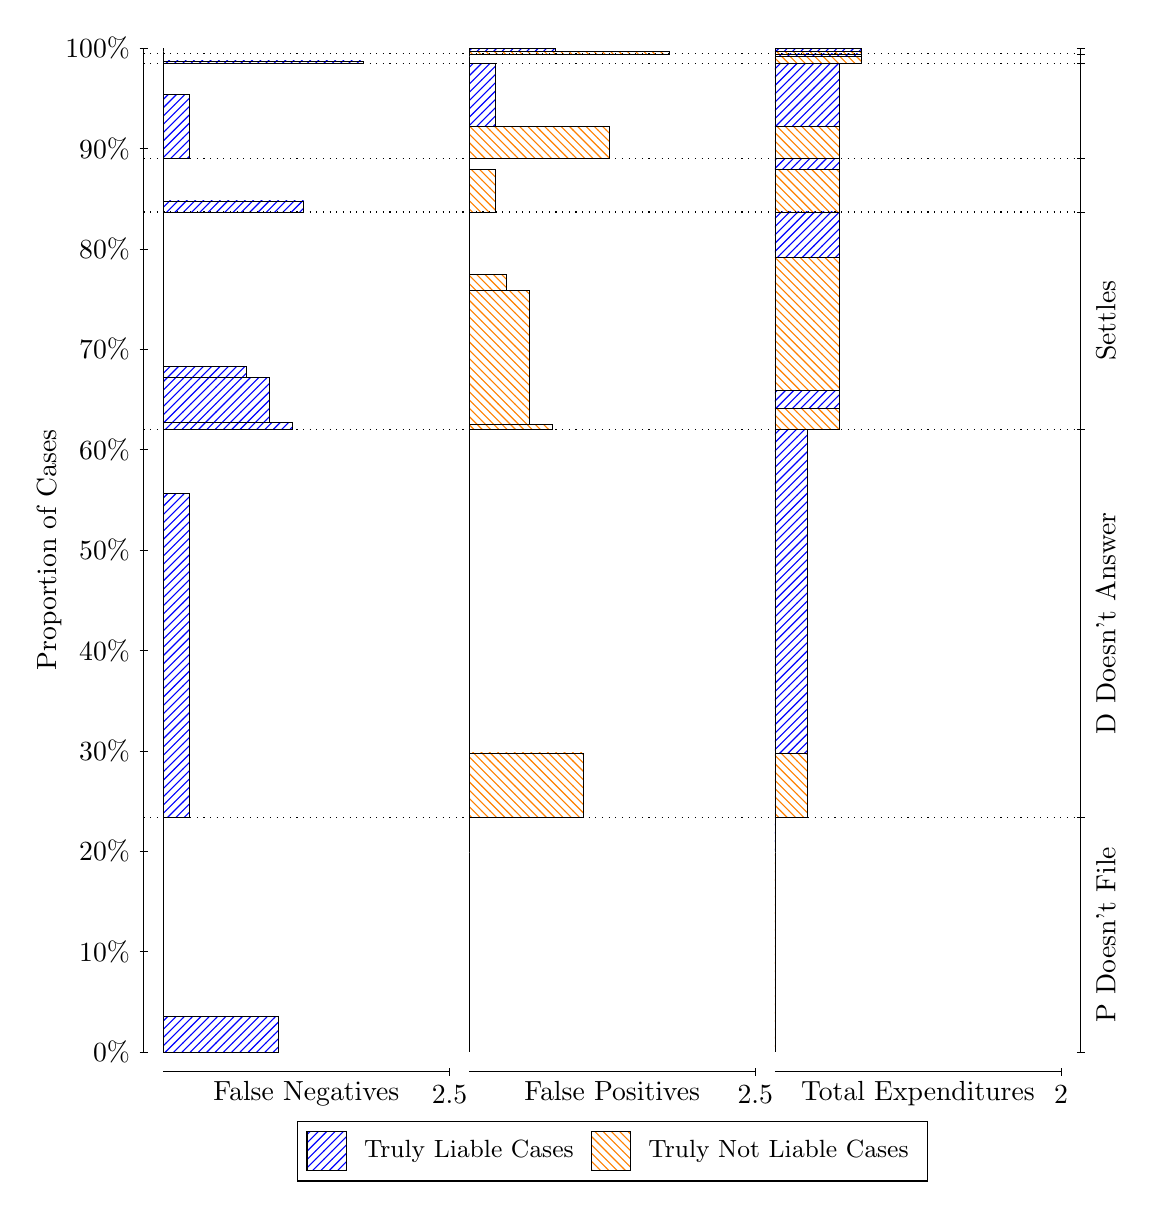
\begin{tikzpicture}
\draw[black, very thin] (1.5,1.75) -- (1.5,14.5);
\node[rotate=90, text=black, anchor=center] at (0.3, 8.125) {Proportion of Cases};
\draw[black, very thin] (1.45,1.75) -- (1.55,1.75);
\node[text=black, anchor=east] at (1.45, 1.75) {0\%};
\draw[black, very thin] (1.45,3.025) -- (1.55,3.025);
\node[text=black, anchor=east] at (1.45, 3.025) {10\%};
\draw[black, very thin] (1.45,4.3) -- (1.55,4.3);
\node[text=black, anchor=east] at (1.45, 4.3) {20\%};
\draw[black, very thin] (1.45,5.575) -- (1.55,5.575);
\node[text=black, anchor=east] at (1.45, 5.575) {30\%};
\draw[black, very thin] (1.45,6.85) -- (1.55,6.85);
\node[text=black, anchor=east] at (1.45, 6.85) {40\%};
\draw[black, very thin] (1.45,8.125) -- (1.55,8.125);
\node[text=black, anchor=east] at (1.45, 8.125) {50\%};
\draw[black, very thin] (1.45,9.4) -- (1.55,9.4);
\node[text=black, anchor=east] at (1.45, 9.4) {60\%};
\draw[black, very thin] (1.45,10.675) -- (1.55,10.675);
\node[text=black, anchor=east] at (1.45, 10.675) {70\%};
\draw[black, very thin] (1.45,11.95) -- (1.55,11.95);
\node[text=black, anchor=east] at (1.45, 11.95) {80\%};
\draw[black, very thin] (1.45,13.225) -- (1.55,13.225);
\node[text=black, anchor=east] at (1.45, 13.225) {90\%};
\draw[black, very thin] (1.45,14.5) -- (1.55,14.5);
\node[text=black, anchor=east] at (1.45, 14.5) {100\%};

\draw[black, very thin] (13.4,1.75) -- (13.4,14.5);
\draw[black, very thin] (13.35,1.75) -- (13.45,1.75);
\node[anchor=west] at (13.35, 1.75) {};
\draw[black, very thin] (13.35,4.7311) -- (13.45,4.7311);
\node[anchor=west] at (13.35, 4.7311) {};
\draw[black, very thin] (13.35,9.6588) -- (13.45,9.6588);
\node[anchor=west] at (13.35, 9.6588) {};
\draw[black, very thin] (13.35,12.418) -- (13.45,12.418);
\node[anchor=west] at (13.35, 12.418) {};
\draw[black, very thin] (13.35,13.102) -- (13.45,13.102);
\node[anchor=west] at (13.35, 13.102) {};
\draw[black, very thin] (13.35,14.307) -- (13.45,14.307);
\node[anchor=west] at (13.35, 14.307) {};
\draw[black, very thin] (13.35,14.425) -- (13.45,14.425);
\node[anchor=west] at (13.35, 14.425) {};
\draw[black, very thin] (13.35,14.5) -- (13.45,14.5);
\node[anchor=west] at (13.35, 14.5) {};

\draw[black, very thin, pattern color=blue, pattern=north east lines] (1.75,1.75) rectangle (3.2033,2.1996);
\draw[black, very thin, pattern color=orange, pattern=north west lines] (1.75,2.1996) rectangle (1.75,4.7311);
\draw[black, very thin, pattern color=blue, pattern=north east lines] (1.75,4.7311) rectangle (2.077,8.8401);
\draw[black, very thin, pattern color=orange, pattern=north west lines] (1.75,8.8401) rectangle (1.75,9.6588);
\draw[black, very thin, pattern color=blue, pattern=north east lines] (1.75,9.6588) rectangle (3.385,9.7469);
\draw[black, very thin, pattern color=blue, pattern=north east lines] (1.75,9.7469) rectangle (3.0943,10.321);
\draw[black, very thin, pattern color=blue, pattern=north east lines] (1.75,10.321) rectangle (2.8037,10.453);
\draw[black, very thin, pattern color=orange, pattern=north west lines] (1.75,10.453) rectangle (1.75,12.418);
\draw[black, very thin, pattern color=blue, pattern=north east lines] (1.75,12.418) rectangle (3.5303,12.559);
\draw[black, very thin, pattern color=orange, pattern=north west lines] (1.75,12.559) rectangle (1.75,13.102);
\draw[black, very thin, pattern color=blue, pattern=north east lines] (1.75,13.102) rectangle (2.077,13.908);
\draw[black, very thin, pattern color=orange, pattern=north west lines] (1.75,13.908) rectangle (1.75,14.307);
\draw[black, very thin, pattern color=blue, pattern=north east lines] (1.75,14.307) rectangle (4.2933,14.337);
\draw[black, very thin, pattern color=orange, pattern=north west lines] (1.75,14.337) rectangle (1.75,14.425);
\draw[black, very thin, pattern color=orange, pattern=north west lines] (1.75,14.425) rectangle (1.75,14.455);
\draw[black, very thin, pattern color=blue, pattern=north east lines] (1.75,14.455) rectangle (1.75,14.5);
\draw[black, very thin, pattern color=orange, pattern=north west lines] (5.6333,1.75) rectangle (5.6333,4.2815);
\draw[black, very thin, pattern color=blue, pattern=north east lines] (5.6333,4.2815) rectangle (5.6333,4.7311);
\draw[black, very thin, pattern color=orange, pattern=north west lines] (5.6333,4.7311) rectangle (7.0867,5.5497);
\draw[black, very thin, pattern color=blue, pattern=north east lines] (5.6333,5.5497) rectangle (5.6333,9.6588);
\draw[black, very thin, pattern color=orange, pattern=north west lines] (5.6333,9.6588) rectangle (6.687,9.7226);
\draw[black, very thin, pattern color=orange, pattern=north west lines] (5.6333,9.7226) rectangle (6.3963,11.419);
\draw[black, very thin, pattern color=orange, pattern=north west lines] (5.6333,11.419) rectangle (6.1057,11.624);
\draw[black, very thin, pattern color=blue, pattern=north east lines] (5.6333,11.624) rectangle (5.6333,12.418);
\draw[black, very thin, pattern color=orange, pattern=north west lines] (5.6333,12.418) rectangle (5.9603,12.961);
\draw[black, very thin, pattern color=blue, pattern=north east lines] (5.6333,12.961) rectangle (5.6333,13.102);
\draw[black, very thin, pattern color=orange, pattern=north west lines] (5.6333,13.102) rectangle (7.4137,13.501);
\draw[black, very thin, pattern color=blue, pattern=north east lines] (5.6333,13.501) rectangle (5.9603,14.307);
\draw[black, very thin, pattern color=orange, pattern=north west lines] (5.6333,14.307) rectangle (5.6333,14.394);
\draw[black, very thin, pattern color=blue, pattern=north east lines] (5.6333,14.394) rectangle (5.6333,14.425);
\draw[black, very thin, pattern color=orange, pattern=north west lines] (5.6333,14.425) rectangle (8.1767,14.455);
\draw[black, very thin, pattern color=blue, pattern=north east lines] (5.6333,14.455) rectangle (6.7233,14.5);
\draw[black, very thin, pattern color=orange, pattern=north west lines] (9.5167,1.75) rectangle (9.5167,4.2815);
\draw[black, very thin, pattern color=blue, pattern=north east lines] (9.5167,4.2815) rectangle (9.5167,4.7311);
\draw[black, very thin, pattern color=orange, pattern=north west lines] (9.5167,4.7311) rectangle (9.9254,5.5497);
\draw[black, very thin, pattern color=blue, pattern=north east lines] (9.5167,5.5497) rectangle (9.9254,9.6588);
\draw[black, very thin, pattern color=orange, pattern=north west lines] (9.5167,9.6588) rectangle (10.334,9.9276);
\draw[black, very thin, pattern color=blue, pattern=north east lines] (9.5167,9.9276) rectangle (10.334,10.148);
\draw[black, very thin, pattern color=orange, pattern=north west lines] (9.5167,10.148) rectangle (10.334,11.844);
\draw[black, very thin, pattern color=blue, pattern=north east lines] (9.5167,11.844) rectangle (10.334,12.418);
\draw[black, very thin, pattern color=orange, pattern=north west lines] (9.5167,12.418) rectangle (10.334,12.961);
\draw[black, very thin, pattern color=blue, pattern=north east lines] (9.5167,12.961) rectangle (10.334,13.102);
\draw[black, very thin, pattern color=orange, pattern=north west lines] (9.5167,13.102) rectangle (10.334,13.501);
\draw[black, very thin, pattern color=blue, pattern=north east lines] (9.5167,13.501) rectangle (10.334,14.307);
\draw[black, very thin, pattern color=orange, pattern=north west lines] (9.5167,14.307) rectangle (10.607,14.394);
\draw[black, very thin, pattern color=blue, pattern=north east lines] (9.5167,14.394) rectangle (10.607,14.425);
\draw[black, very thin, pattern color=orange, pattern=north west lines] (9.5167,14.425) rectangle (10.607,14.455);
\draw[black, very thin, pattern color=blue, pattern=north east lines] (9.5167,14.455) rectangle (10.607,14.5);
\draw[black, dotted] (1.5,4.7311) -- (13.4,4.7311);
\draw[black, dotted] (1.5,9.6588) -- (13.4,9.6588);
\draw[black, dotted] (1.5,12.418) -- (13.4,12.418);
\draw[black, dotted] (1.5,13.102) -- (13.4,13.102);
\draw[black, dotted] (1.5,14.307) -- (13.4,14.307);
\draw[black, dotted] (1.5,14.425) -- (13.4,14.425);
\draw[black, very thin] (1.75,1.5) -- (5.3833,1.5);
\node[text=black, anchor=north] at (3.5667, 1.5) {False Negatives};
\draw[black, very thin] (5.3833,1.45) -- (5.3833,1.55);
\node[text=black, anchor=north] at (5.3833, 1.45) {2.5};

\draw[black, very thin] (5.6333,1.5) -- (9.2667,1.5);
\node[text=black, anchor=north] at (7.45, 1.5) {False Positives};
\draw[black, very thin] (9.2667,1.45) -- (9.2667,1.55);
\node[text=black, anchor=north] at (9.2667, 1.45) {2.5};

\draw[black, very thin] (9.5167,1.5) -- (13.15,1.5);
\node[text=black, anchor=north] at (11.333, 1.5) {Total Expenditures};
\draw[black, very thin] (13.15,1.45) -- (13.15,1.55);
\node[text=black, anchor=north] at (13.15, 1.45) {2};

\node[text=black, centered, rotate=90] at (13.72, 3.2406) {P Doesn't File};
\node[text=black, centered, rotate=90] at (13.72, 7.1949) {D Doesn't Answer};
\node[text=black, centered, rotate=90] at (13.72, 11.038) {Settles};





\draw (7.449999999999999,1.5) node[draw=none] (baseCoordinate) {};
\begin{scope}[align=center]
        \matrix[scale=0.5, draw=black, below=0.5cm of baseCoordinate, nodes={draw}, column sep=0.1cm]{
            \node[rectangle, draw, minimum width=0.5cm, minimum height=0.5cm, pattern color=blue, pattern=north east lines] {}; &
            \node[draw=none, font=\small, text=black] (B) {Truly Liable Cases}; &
            \node[rectangle, draw, minimum width=0.5cm, minimum height=0.5cm, pattern color=orange, pattern=north west lines] {}; &
            \node[draw=none, font=\small, text=black] (B) {Truly Not Liable Cases}; \\
            };
\end{scope}

\end{tikzpicture}
\end{document}